\documentclass[12pt]{article}
%\usepackage[utf8]{inputenc}
\usepackage[margin=1in]{geometry}
\usepackage{amsmath, amssymb}
\usepackage{hyperref, listings}
\usepackage{systeme}
\usepackage{listings}
\usepackage{comment}
\usepackage{enumitem}
%\usepackage[version=4]{mhchem}


% Toggle for which version to print
% A bit hacky, there must be a nicer way of doing this...
\usepackage{ifthen}

% Use single counter for problems
\newcounter{ProblemCounter}



\usepackage{pgf,tikz}
\usetikzlibrary{arrows, automata, positioning}
\lstset{numbers=left, numberstyle=\small, numbersep=8pt, frame = single, framexleftmargin=15pt}

\pgfdeclarelayer{nodelayer}
\pgfdeclarelayer{edgelayer}
\pgfsetlayers{edgelayer,nodelayer,main}


% Uncomment next line to compile with solutions
%\def\solutions{1}

\ifx\solutions\undefined
\newcommand{\sol}[1]{}
\else
\newcommand{\sol}[1]{{\color{red} \textbf{Solution: } #1}}
\fi






\tikzset{newstyle/.style={thick}}
\tikzset{simple/.style={thick}}

%% PP
\newcommand{\todo}[1]{\vspace{5 mm}\par \noindent \marginpar{\textsc{ToDo}}
\framebox{\begin{minipage}[c]{0.95 \linewidth}
\tt #1 \end{minipage}}\vspace{5 mm}\par}
\newcommand{\R}{{\mathbb R}}
\newcommand{\C}{{\mathbb C}}
\newcommand{\Z}{{\mathbb Z}}
\newcommand{\Q}{{\mathbb Q}}
\newcommand{\N}{{\mathbb N}}
\newcommand{\norm}[1]{\left\lVert#1\right\rVert}
%%
%% CY
\newcommand{\bmat}[1]{\begin{bmatrix}#1\end{bmatrix}}
\newcommand{\abs}[1]{\left| #1 \right|}
\newcommand{\dotp}[1]{\left\langle #1 \right\rangle}
\DeclareMathOperator{\rank}{rank}
\DeclareMathOperator{\proj}{proj}
\DeclareMathOperator{\spann}{span}
%%


\title{18.C21 Practice Midterm \\
Spring 2026 (Johnson \& Marzouk)
\ifdefined\solutions
--- \textcolor{red}{Solutions}
\fi
}
\author{}
\date{}
\begin{document}

\maketitle

\ifx\solutions\undefined

% Signature line
{\vspace{1.2cm} \hspace{1cm}
{\Large \textbf{NAME:} \dotfill}
\hspace{2cm}\ \vspace{1cm}}

\fi

\begin{itemize}

\item The practice exam is likely to be both \textbf{harder} and \textbf{longer} than the real exam.

\item You will have \textbf{50 minutes} after your exam begins.

\item Write your \textbf{NAME} above \emph{and} at the top of \emph{every} page. Please do it as soon as you begin the exam, and check again before returning it. 

\item Only write on \emph{one} side of each sheet.  Additional paper will be provided upon request.

\item You can bring \textbf{1 letter-sized sheet of notes} (both sides if you want), though it is unlikely to help much.

\item
\textbf{Please allocate your time carefully}, to make sure you get to work on all parts.  Take a quick look at the \emph{whole exam}, before starting working on your first problem.

\item \textbf{Show your work / justify your answers.}  Wrong answers may still receive partial credit \emph{if} the reasoning was somewhat correct.

\item If you absolutely believe there is something wrong with a problem, please ask. No hints, other than the ones already written in the exam, will be given.

%\item Once you are done, or the \textbf{2-hour exam time} is up, please upload your file in \textbf{Gradescope}. Again, please make sure you write your name in every page.

\end{itemize}

%%%%%%%%%%%%%%%%%%%%%%%%%%%%%%%%%%%%%%%%%%%%%%%%%%%%%%%%%

\newpage
\section*{Problem 1}

Recall that double-precision (\texttt{Float64}) floating-point numbers store about 15--16 decimal significant digits, and can represent magnitudes from around $\approx 10^{-300}$ to around $\approx 10^{300}$ (after which they under/overflow, respectively).

\begin{enumerate} \item Many libraries, including SciPy, provide a function $\operatorname{logsumexp}(x)$ which takes a vector $x \in \R^n$ and computes the mathematical function:
$$
\operatorname{logsumexp}(x) = \log\left(\sum_{i=1}^n e^{x_i} \right) \, .
$$
Explain why, for accuracy reasons (ignoring performance), this function should \emph{not} be implemented naively using the above formula (e.g.~\emph{don't} do \texttt{log(sum(exp.(x)))} in Julia or \texttt{numpy.log(numpy.sum(numpy.exp(x)))} in Python).  In fact, there are \emph{two} extremes in which the naive formula goes horribly wrong and gives no correct digits in floating-point arithmetic.  What are they?  (Hint: think about $\max_i x_i$).
\item Outline (as pseudo-code) the steps of an modified algorithm to compute the same function without the catastrophes identified in the previous part.  (Hint: factor something out of the sum, and remember the identity $\log(ab) = \log a+\log b$.)
\end{enumerate}

\sol{Answer 1.
}
\vfill

\newpage
$\mbox{}$
\newpage

\section*{Problem 2}

The ``error'' function $\operatorname{erf}(x) = \frac{2}{\sqrt \pi}\int_0^x e^{-t^2}\,dt$ is a standard special function (provided by many libraries, such as \texttt{scipy.special.erf}) that computes \emph{part} of a Gaussian integral.  It is plotted in Fig.~\ref{fig:erf} and has the property that $\operatorname{erf}(x)\to 1$ exponentially fast as $x \to \infty$, because $\int_0^\infty e^{-t^2}\,dt = \sqrt{\pi}/2$ (the famous ``Gaussian integral'').

\begin{figure}[b!]
    \centering
    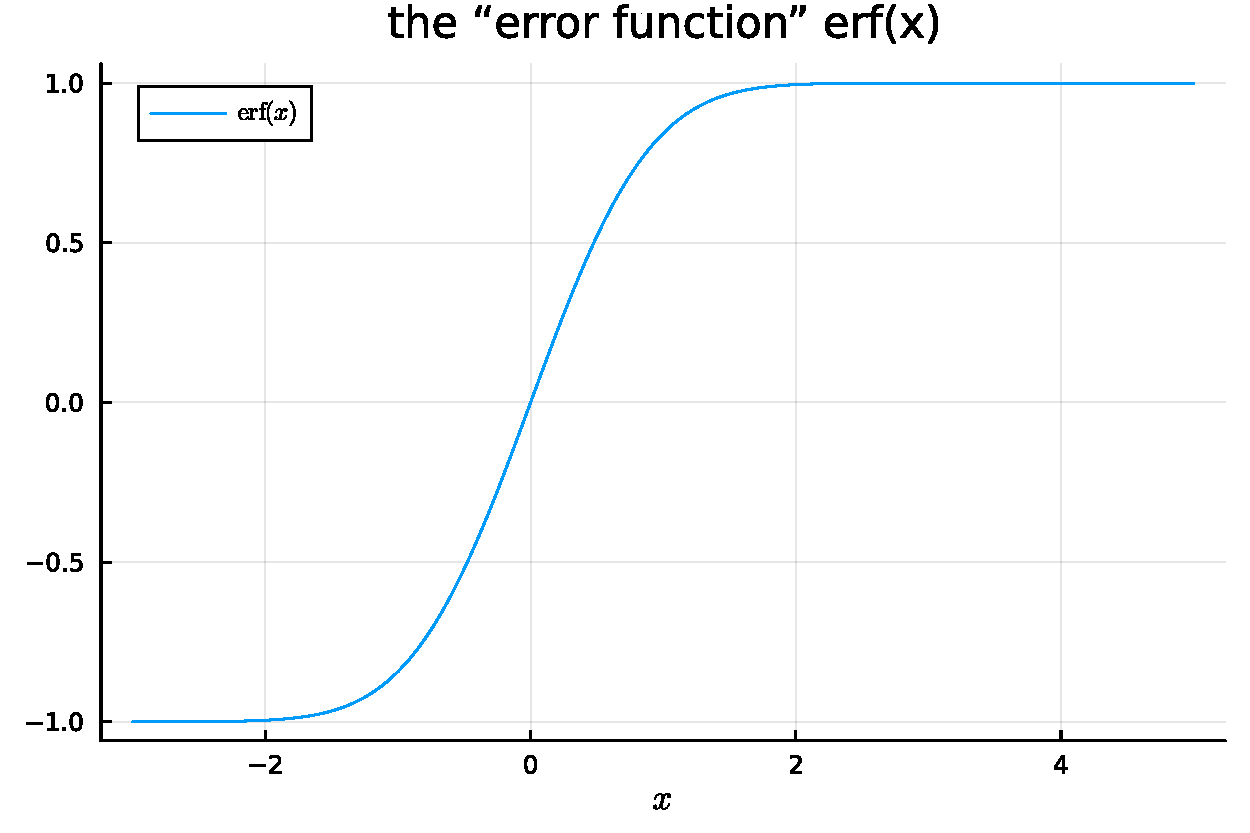
\includegraphics[width=0.7\textwidth]{erf.pdf}
    \caption{Plot of the error function $\operatorname{erf}(x)$.}
    \label{fig:erf}
\end{figure}

\begin{enumerate}
    \item The same libraries \emph{also} provide a function $\operatorname{erfc}(x) = 1 - \operatorname{erf}(x)$, the ``complementary error function.''  Why?  Aren't $\operatorname{erf}$ and $\operatorname{erfc}$ redundant?  Why information would you potentially lose if you simply subtract $\operatorname{erf}$ from $1$ yourself?  Conversely, given $\operatorname{erfc}$, why do you still need $\operatorname{erf}$ if you want don't want to lose information for some inputs, rather than using $\operatorname{erf}(x) = 1 - \operatorname{erfc}(x)$?


    \newpage

    \item For large $x \gg 1$, the error function is approximately $\operatorname{erf}(x) \approx 1 - e^{-x^2} / (x\sqrt{\pi})$.  Use this to compute the relative condition number $\kappa_r(\operatorname{erfc}, x)$ for large $x \gg 1$.  And by inspection of the plot (of $\operatorname{erf}$), what is the relative condition number of $\operatorname{erfc}$ (not $\operatorname{erf}$) as $x \to 0$?
    
    \textit{Comment:} These results explain why there should be an algorithm to compute $\operatorname{erfc}$ accurately when $\operatorname{erf}(x)$ is close to $1$, despite the problem you identified with the naive formula in the previous part.   
    
    (Recall that for any differentiable scalar function $f(x)$, $\kappa_r(f, x) = |f'(x)|\frac{|x|}{|f(x)|}$.  Also recall the fundamental theorem of calculus, saying that the derivative is the inverse of integration: $(\int^x g(t)\, dt)' = g(x)$.)
    \vfill

    \item $\operatorname{erf}$ is the integral of a smooth function $e^{-t^2}$, so you can compute it yourself for any given $x$ very accurately with quadrature schemes like Clenshaw--Curtis (with errors that decrease at least exponentially fast with the number of quadrature points $t$).   However, if we wanted to evaluate the function $\operatorname{erf}(x)$ for many different $x$ values (and let's pretend you don't have a library function like \texttt{scipy.special.erf} available), say for $x \in [-10,10]$, outline (as a sequence of steps) how you might construct an approximation $a(x)$ for $\operatorname{erf}(x)$ on $[-10,10]$ such that (after the construction) the resulting $a(x)$ can then be evaluated quickly and accurately (to, say, at least 10 digits) for any given value of $x$, probably more quickly than re-doing quadrature for each $x$? 
\end{enumerate}


\sol{Answer 2.

}
\vfill


\newpage

%%%%%%%%%%%%%%%

\section*{Problem 3}

In Fig.~\ref{convergence}(left) are shown three functions $f_1(x)$, $f_2(x)$, and $f_3(x)$ on $x\in[0,1]$.  On the right are shown the convergence of Clenshaw--Curtis quadrature to compute $\int_0^1 f_i(x)\,dx$ for $n+1$ point versus $n$ for these three functions, labeled $A,B,C$, but we do \emph{not} tell you which of $f_1,f_2,f_3$ are referred to by $A,B,C$.


\begin{figure}[b!]
    \centering
    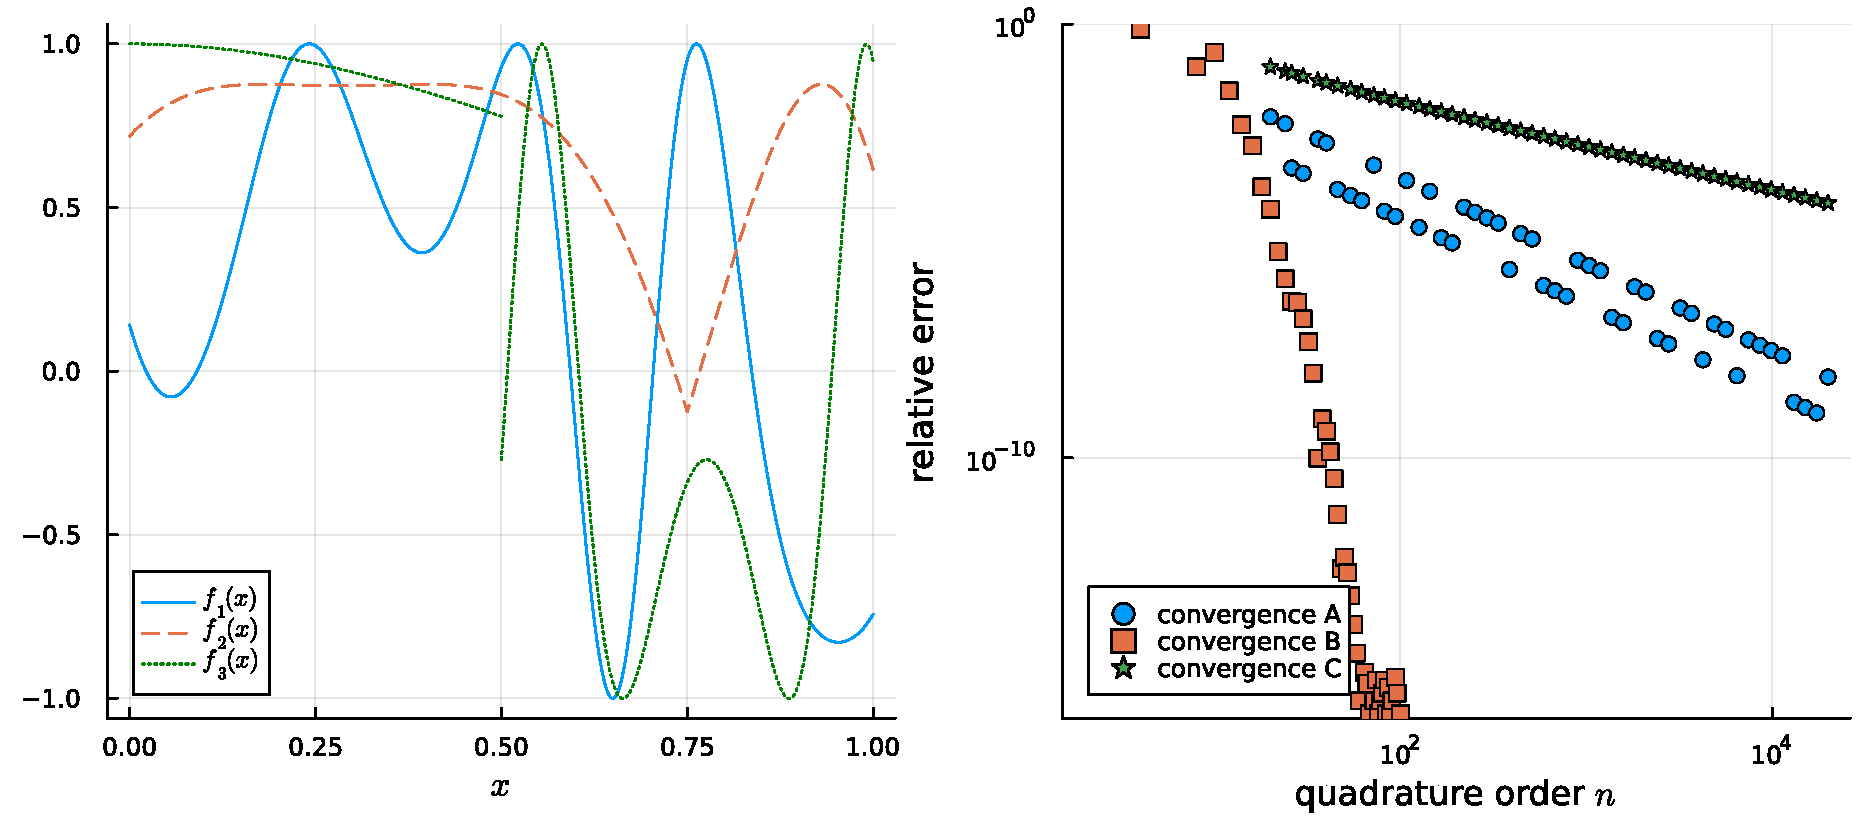
\includegraphics[width=0.7\textwidth]{convergence-3.pdf}
    \caption{Plot of three functions $f_1(x)$, $f_2(x)$, and $f_3(x)$ on $x\in[0,1]$ (left), and the convergence versus Clenshaw--Curtis quadrature order $n$ ($n+1$ points) for these three functions, but in an unspecified order.}
    \label{fig:convergence}
\end{figure}


\begin{enumerate}
\item Which function in Fig.~\ref{convergence}(left) correspond to which convergence curve in Fig.~\ref{convergence}(right), and why?  Give a few words of justification, no formal analysis required.
\vfill
\item For the two functions that are converging slowly in Fig.~\ref{convergence}(right), explain how you might modify your integration algorithm (given a function that does Clenshaw--Curtis quadrature on any desired interval $[a,b]$ for any $n$) to get fast convergence for these two cases. 
\vfill
\end{enumerate}

\sol{
\begin{enumerate}
\item answer 1
\item answer 2
\end{enumerate}
}
\newpage
$\mbox{}$
\newpage

%%%%%%%%%%%%%%%
\section*{Problem 4}

In problem set~1, you found that the quadratic curve $q(x)$ that goes through the three points $(0,f(0))$ and $(\pm \Delta x, f(\pm \Delta x))$ is:
$$
q(x) = \frac{1}{2\Delta x^2} \left[ f(-\Delta x) x(x - \Delta x) - 2f(0) (x^2 - \Delta x^2) + f(+\Delta x) x(x+ \Delta x) \right]
$$
Explain how you would use this to \textbf{derive a quadrature rule} to estimate the integral
$$
\int_{-\Delta x}^{+\Delta x} f(x)\, dx \approx w_1 f(-\Delta x) + w_2 f(0) + w_3 f(+\Delta x) \, ,
$$
similar to how we derived the trapezoidal rule in class.  \textbf{Give the weights} $w_1,w_2,w_3$.  (This is called ``Simpson's rule.'')

\sol{Answer 4.
}

\newpage

%%%%%%%%%%%%%%%%%%%%%%%%
\section*{Problem 5}

Suppose that we have 100 measurements $(p_{k},v_{k})$ of the volume $v$ of a gas vs.~its pressure $p$, and we want to fit it to a function of the form $v(p)=\frac{c_{1}}{p}+c_{2}$ for unknown constants $c_{1},c_{2}$. Write down a $2\times2$ system of equations you could solve to find $c_{1},c_{2}$ in order to minimize the sum of the squared errors $\sum_{k}[v(p_{k})-v_{k}]^{2}$. You can write your answer (left- and right-hand sides) as products of matrices and/or vectors, as long as you specify what each term is (in terms of the unknowns $c_{1},c_{2}$ and/or the data $p_{1},\ldots,p_{100}$ and $v_{1},\ldots,v_{100})$.

(Recall that for least-square problems $\min_x \Vert Ax - b\Vert_2$ we derived the normal equations $A^T Ax=A^T b$ for the minimizer $x$, though we will see that there are often better ways to solve such problems.)

\sol{This is a least-square problem, so the answer is
to solve the normal equations $\boxed{A^{T}Ac=A^{T}b}$ for $c=\left(\begin{array}{cc}
c_{1} & c_{2}\end{array}\right)^{T}$ where 
\[
\boxed{A=\left(\begin{array}{cc}
\frac{1}{p_{1}} & 1\\
\frac{1}{p_{2}} & 1\\
\vdots & \vdots\\
\frac{1}{p_{100}} & 1
\end{array}\right)}\text{ and }\boxed{b=\left(\begin{array}{c}
v_{1}\\
v_{2}\\
\vdots\\
v_{100}
\end{array}\right)}
\]
so that $Ac$ is the ``model'' $\left(\begin{array}{c}
v(p_{1})\\
v(p_{2})\\
\vdots\\
v(p_{100})
\end{array}\right)$ and $b$ are the data we are fitting to, so that $\sum_{k}[v(p_{k})-v_{k}]^{2}=\Vert Ac-b\Vert^{2}$. 
}

\end{document}
